\documentclass{beamer}
% Some basic packagesLLuu
\usepackage[utf8]{inputenc}
\usepackage{spverbatim}
\usepackage{textcomp}
\usepackage{pgfplots}
\usepackage{url}
\usepackage{graphicx}
\usepackage{float}
\usepackage{algorithm2e}
\usepackage{enumitem}
\usepackage{standalone}
\usepackage{tcolorbox}
\usepackage{wrapfig}
% \usepackage{svg}
% \usepackage{svg-inkscape} 

\graphicspath{{./figures}}

%color settings
\usepackage{xcolor}
\definecolor{gruvbgdark}{HTML}{1d2021}
\definecolor{gruvtextdark}{HTML}{ebdbb2}
\definecolor{gruvbglight}{HTML}{f9f5d7}
\definecolor{gruvtextlight}{HTML}{3c3836}
\definecolor{NavyBlue}{HTML}{266bbd}
\definecolor{RawSienna}{HTML}{94330e}
\definecolor{ForestGreen}{HTML}{149b52}
% \pagecolor{gruvbgdark}
% \color{gruvtextdark}

% Hide page number when page is empty
\usepackage{emptypage}
\usepackage{subcaption}
\usepackage{multicol}

% Math stuff
\usepackage{amsmath, amsfonts, mathtools, amsthm, amssymb}
% Fancy script capitals
\usepackage{mathrsfs}
\usepackage{cancel}

% Bold math
\usepackage{bm}

%Algorithm setup
\RestyleAlgo{algoruled}
% Some shortcuts
\newcommand\N{\ensuremath{\mathbb{N}}}
\newcommand\R{\ensuremath{\mathbb{R}}}
\newcommand\Z{\ensuremath{\mathbb{Z}}}
\renewcommand\O{\ensuremath{\emptyset}}
\newcommand\Q{\ensuremath{\mathbb{Q}}}
\newcommand\C{\ensuremath{\mathbb{C}}}
\newcommand\B{\ensuremath{\mathbb{B}}}

%Make implies and impliedby shorter
\let\implies\Rightarrow
\let\impliedby\Leftarrow
\let\iff\Leftrightarrow

\let\epsilon\varepsilon

% Add \contra symbol to denote contradiction
% \usepackage{stmaryrd} % for \lightning
% \newcommand\contra{\scalebox{1.5}{$\lightning$}}

\let\phi\varphi

% Command for short corrections
% Usage: 1+1=\correct{3}{2}

\definecolor{correct}{HTML}{009900}
\newcommand\correct[2]{\ensuremath{\:}{\color{red}{#1}}\ensuremath{\to }{\color{correct}{#2}}\ensuremath{\:}}
\newcommand\green[1]{{\color{correct}{#1}}}

% horizontal rule
% \newcommand\hr{
%     \noindent\rule[0.5ex]{\linewidth}{0.5pt}
% }

% hide parts
\newcommand\hide[1]{}

% Environments
\makeatother


\newcommand{\oefening}[1]{%
	\def\@oefening{#1}%
	\subsection*{Oefening #1}
}

\newcommand{\suboefening}[1]{%
	\subsubsection*{Oefening \@oefening.#1}
}


% \lecture starts a new lecture (les in dutch)
%
% Usage:
% \lecture{1}{di 12 feb 2019 16:00}{Inleiding}
%
% This adds a section heading with the number / title of the lecture and a
% margin paragraph with the date.

% I use \dateparts here to hide the year (2019). This way, I can easily parse
% the date of each lecture unambiguously while still having a human-friendly
% short format printed to the pdf.

% \usepackage{xifthen}
% \def\testdateparts#1{\dateparts#1\relax}
% \def\dateparts#1 #2 #3 #4 #5\relax{
% 	\marginpar{\small\textsf{\mbox{#1 #2 #3 #5}}}
% }

% \def\@lecture{}%
% \newcommand{\lecture}[3]{
% 	\ifthenelse{\isempty{#3}}{%
% 		\def\@lecture{Lecture #1}%
% 	}{%
% 		\def\@lecture{Lecture #1: #3}%
% 	}%
% 	\subsection*{\@lecture}
% 	% \marginpar{\small\textsf{\mbox{#2}}}
% }

\usepackage{listings}

\definecolor{dkgreen}{rgb}{0,0.6,0}
\definecolor{gray}{rgb}{0.5,0.5,0.5}
\definecolor{mauve}{rgb}{0.58,0,0.82}

\lstset{frame=none,
  language=python,
  aboveskip=3mm,
  belowskip=3mm,
  showstringspaces=false,
  columns=flexible,
  basicstyle={\small\ttfamily},
  numbers=none,
  numberstyle=\tiny\color{gray},
  keywordstyle=\color{blue},
  commentstyle=\color{dkgreen},
  stringstyle=\color{mauve},
  breaklines=true,
  breakatwhitespace=true,
  tabsize=3
}



% These are the fancy headers

% LE: left even
% RO: right odd
% CE, CO: center even, center odd
% My name for when I print my lecture notes to use for an open book exam.

\makeatother

\usepackage{tcolorbox}

% Make boxes breakable
\tcbuselibrary{breakable}

% Figure support as explained in my blog post.
\usepackage{import}
\usepackage{xifthen}
\usepackage{pdfpages}
\usepackage{transparent}
\newcommand{\incfig}[2][1]{%
	% \begin{center}
	\def\svgwidth{#1\columnwidth}
	\import{./figures/}{#2.pdf_tex}
	% \end{center}
}
% Fix some stuff
% %http://tex.stackexchange.com/questions/76273/multiple-pdfs-with-page-group-included-in-a-single-page-warning
\pdfsuppresswarningpagegroup=1
\author{Kristian Sørdal}

%Information to be included in the title page:
\title{Parallell Matrix Vector Multiplier - Results}
\author{Kristian Sørdal}
\institute{University of Bergen}

\begin{document}

\frame{\titlepage}

\begin{frame}
\frametitle{Total time - Task A and Sequential}
\begin{figure}
  \centering
  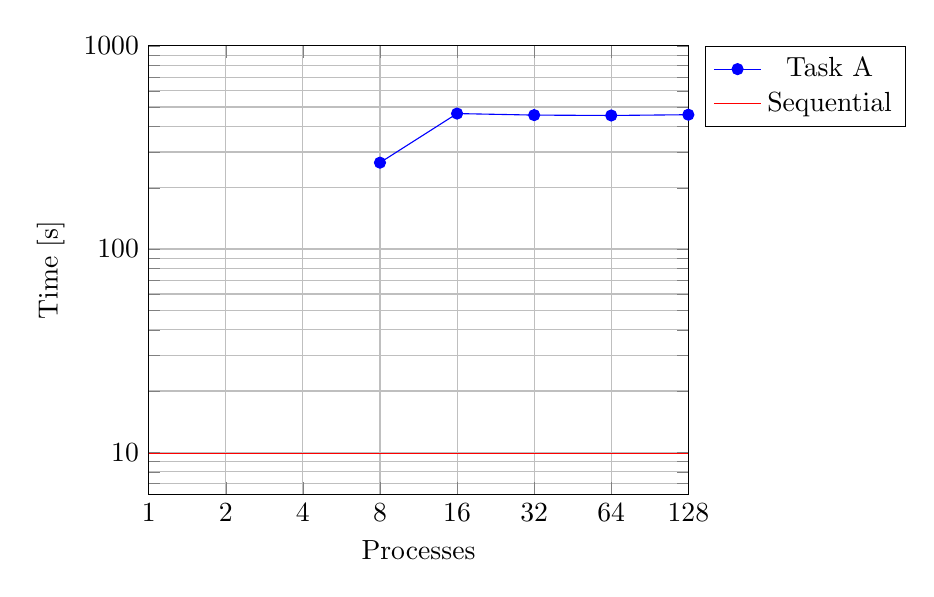
\begin{tikzpicture}
    \begin{axis}[
        xlabel={Processes},
        ylabel={Time [s]},
        legend pos=outer north east, % Adjust the legend position
        grid=both, % Display grid lines
        xmode=log, % Set x-axis to logarithmic scale
        ymode=log,
        xmin=1, xmax=128, % Set x-axis limits
        ymin=0, ymax=1000, % Set y-axis limits
        xtick={1,2,4,8,16,32,64,128}, % Specify the x-axis tick values
        ytick={0.1,0.2,0.3,0.4,0.5,0.6,0.7,0.8,0.9,1,2,3,4,5,6,7,8,9,10,20,30,40,50,60,70,80,90,100,200,300,400,500,600,700,800,900,1000}, 
        yticklabels={0.1,\phantom{a},\phantom{a},\phantom{a},\phantom{a},\phantom{a},\phantom{a},\phantom{a},\phantom{a},1,\phantom{a},\phantom{a},\phantom{a},\phantom{a},\phantom{a},\phantom{a},\phantom{a},\phantom{a},10,\phantom{a},\phantom{a},\phantom{a},\phantom{a},\phantom{a},\phantom{a},\phantom{a},\phantom{a},100,\phantom{a},\phantom{a},\phantom{a},\phantom{a},\phantom{a},\phantom{a},\phantom{a},\phantom{a},1000}, 
        xticklabels={1,2,4,8,16,32,64,128}, % Specify the labels for the tick values
      ]
      
      % Line 1
      \addplot[blue, mark=*, mark options={blue}] coordinates {
              (8,266)
              (16,464)
              (32,456)
              (64,454)
              (128,458)
      };
      \addlegendentry{Task A}
      \addplot[red] coordinates {
              (1,9.86)
              (128,9.86)
      };
      \addlegendentry{Sequential}
     
     
    \end{axis}
  \end{tikzpicture}
  \caption{Total time - scale 12}
\end{figure}

\end{frame}
\begin{frame}
\frametitle{Results of communication times}
\begin{figure}
  \centering
  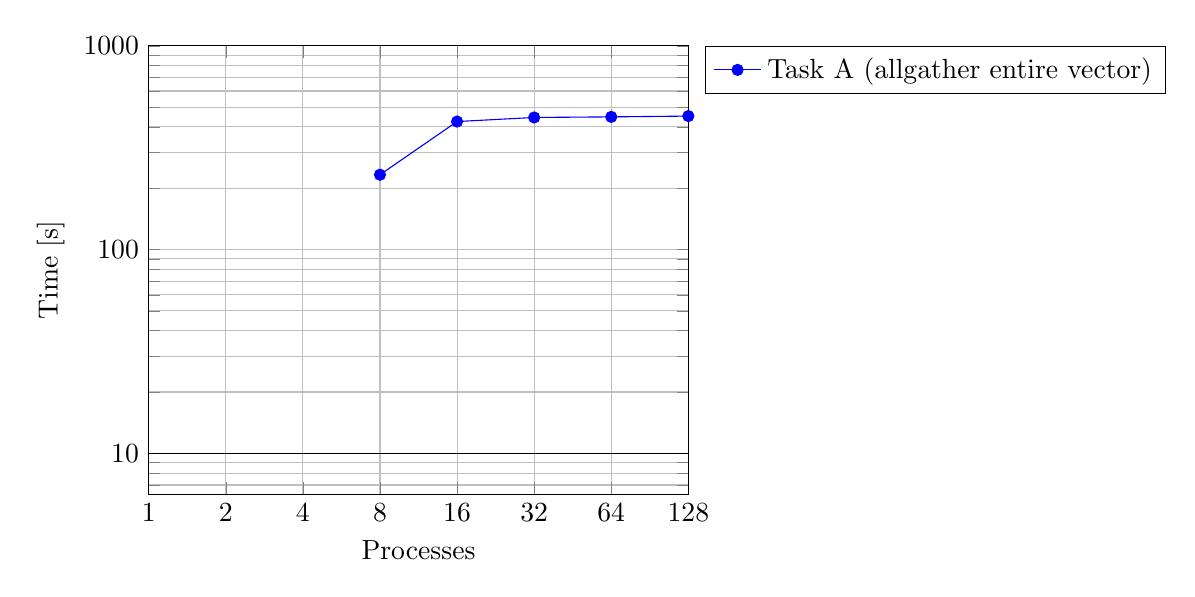
\begin{tikzpicture}
    \begin{axis}[
        xlabel={Processes},
        ylabel={Time [s]},
        legend pos=outer north east, % Adjust the legend position
        grid=both, % Display grid lines
        xmode=log, % Set x-axis to logarithmic scale
        ymode=log,
        xmin=1, xmax=128, % Set x-axis limits
        ymin=0, ymax=1000, % Set y-axis limits
        xtick={1,2,4,8,16,32,64,128}, % Specify the x-axis tick values
        ytick={0.1,0.2,0.3,0.4,0.5,0.6,0.7,0.8,0.9,1,2,3,4,5,6,7,8,9,10,20,30,40,50,60,70,80,90,100,200,300,400,500,600,700,800,900,1000}, 
        yticklabels={0.1,\phantom{a},\phantom{a},\phantom{a},\phantom{a},\phantom{a},\phantom{a},\phantom{a},\phantom{a},1,\phantom{a},\phantom{a},\phantom{a},\phantom{a},\phantom{a},\phantom{a},\phantom{a},\phantom{a},10,\phantom{a},\phantom{a},\phantom{a},\phantom{a},\phantom{a},\phantom{a},\phantom{a},\phantom{a},100,\phantom{a},\phantom{a},\phantom{a},\phantom{a},\phantom{a},\phantom{a},\phantom{a},\phantom{a},1000}, 
        xticklabels={1,2,4,8,16,32,64,128}, % Specify the labels for the tick values
      ]
      
      % Line 1
      \addplot[blue, mark=*, mark options={blue}] coordinates {
              (8,233)
              (16,425)
              (32,445)
              (64,448)
              (128,452)
      };
      \addlegendentry{Task A (allgather entire vector)}
      \addplot[black] coordinates {
              (1,10)
              (128,10)
      };
      
     
    \end{axis}
  \end{tikzpicture}
  \caption{Communication Time - scale 12}
\end{figure}
\end{frame}

\begin{frame}
\frametitle{GFLOPS}
\begin{figure}
\centering
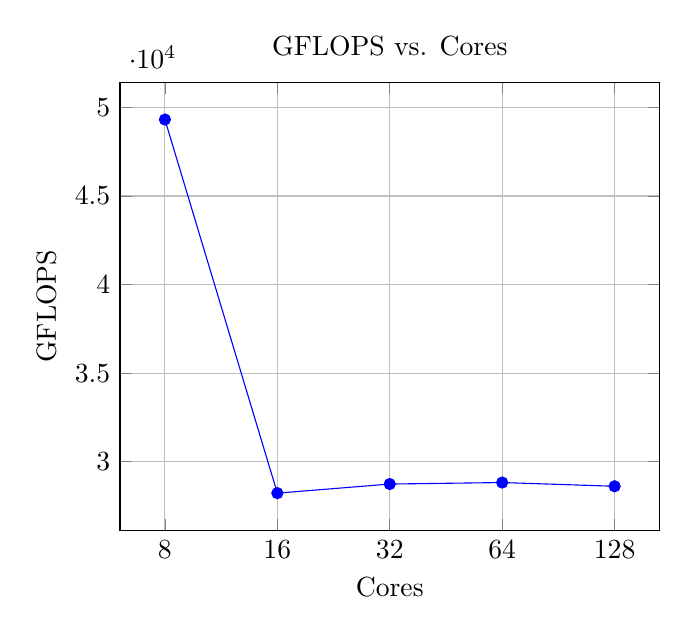
\begin{tikzpicture}
\begin{axis}[
    title={GFLOPS vs. Cores},
    xmode=log, % Set x-axis to logarithmic scale
    xlabel={Cores},
    ylabel={GFLOPS},
    xtick={1,2,4,8,16,32,64,128},
    xticklabels={1,2,4,8,16,32,64,128},
    grid=major,
]

\addplot[color=blue, mark=*] coordinates {
    (8, 49316.6)
    (16, 28227.4)
    (32, 28741.1)
    (64, 28826.3)
    (128, 28616.6)
};
\end{axis}
\end{tikzpicture}
\caption{GFLOPS for Different Numbers of Cores}
\end{figure}
\end{frame}
\begin{frame}
\frametitle{L2 Norm}
\begin{figure}
\centering
\begin{tikzpicture}
\begin{axis}[
    ybar,
    xmode=log,
    xlabel={Cores},
    ylabel={L2},
    xtick={1,2,4,8,16,32,64,128},
    xticklabels={1,2,4,8,16,32,64,128},
]

\addplot[color=blue, mark=*] coordinates {
    (8, 0.973794)
    (16, 1.37715)
    (32, 2.75431)
    (64, 3.89518)
    (128, 3.89518)
};
\end{axis}
\end{tikzpicture}
\caption{GFLOPS for Different Numbers of Cores}
\end{figure}
\end{frame}

\begin{frame}
    \frametitle{What went wrong?}

    \begin{itemize}
        \item The code I wrote was unnecesarily complex, resulted in a lot of mental overhead when coding. 
        \item Poor time management. Spent too much time trying to fix task B, which was ultimately unsuccesful. Resulted in less time for the other tasks.
        \item Didn't spend enough time testing on EX3 at higher scales, which made me believe the code work, even though it didn't.
        \item Task D: deadlocks when waiting for communcation of send lists at scale \( > 9 \)
        \item Lesson learned: Work on other tasks when stuck. Test earlier on EX3. Write simpler code.
    \end{itemize}
\end{frame}
\end{document}

